\section{The \SYSTEM{} Approach} \label{sec:approach}

In this section we detail the \SYSTEM{} approach: a practical defense against
receiving corrupted or compromised resources over the internet. We further
present our Google Chrome extension implementations, \DNSSYS{} and \DHTSYS{}.

The \SYSTEM{} approach can be incorporated into software on most any device
capable of communicating with a chosen backend. This includes desktops, laptops,
tablets, mobile devices, embedded systems, etc.

\subsection{Defeating User Apathy}

Human factors such as user apathy have stymied cryptographers for decades.
Schemes that are otherwise reasonably cryptographically solid can fail
catastrophically due to human error, confusion, or simple lack of interest. Some
users are likely to avoid using a security measure altogether if it presents
even a minor obstacle to immediate gratification~\cite{Clickthrough, PGPBad}. In
the browser, for example, this phenomenon can be observed empirically.

\PUNT{\begin{figure}[t]
    \centering
    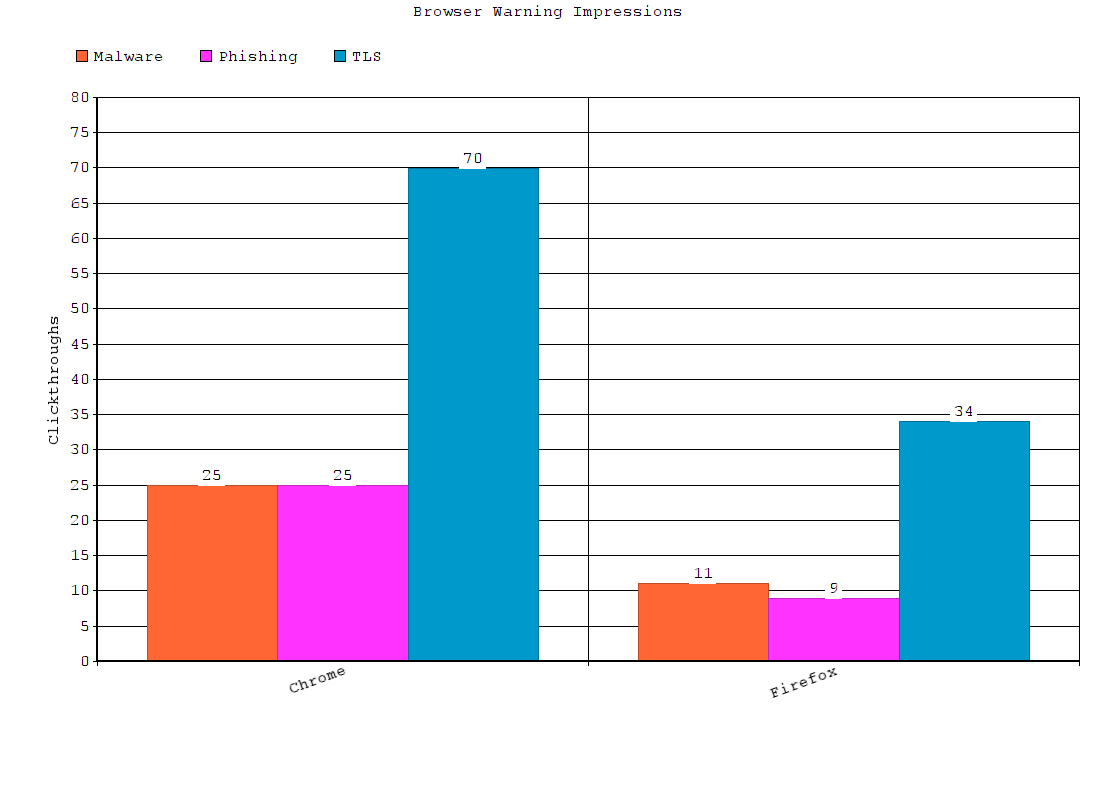
\includegraphics[width=0.95\linewidth]{impressions.png}
    \caption{Akhawe et al. estimation of warning clickthroughs by users as a
    percentage of total warnings observed for two popular
    browsers.}\label{fig:telemetry}
\end{figure}}

Leveraging the in-browser telemetry of Mozilla Firefox and Google Chrome to
passively observe over 25 million warning impressions in 2013, Akhawe et al.
found that users of Google Chrome clicked through a \emph{quarter of malware and
phishing warnings} and \emph{70\% of TLS warnings}~\cite{Clickthrough}. Users
also clicked through a third of Mozilla Firefox's TLS warnings and a tenth of
their malware and phishing warnings. That is to say: a significant percentage of
browser users are \emph{determined} not to let TLS trust issues and/or the
threat of malware prevent them from receiving their desired content. Hence, we
must assume: some non-trivial number of users, similarly determined to transact
resources over the internet, will not be burdened with the off-path minutiae of
manually calculating a checksum (if they are even familiar with the jargon) and
verifying the integrity of the resources they are downloading.

With this assumption in mind, the primary goal of \SYSTEM{} then is to side-step
the human factor altogether by providing a completely transparent and
unobtrusive in the average case, fully-automated method of checksum calculation
and verification in the average case that requires no changes to application
logic or source code. We achieve this through 1) the unique identification of
individual hosted resources and 2) a high availability mapping of unique
resource identifiers to corresponding checksums.

\SYSTEM{} implementations can be imagined as a security layer sitting between
the user and the resource. Immediately after a resource is downloaded, two
cryptographic digests are generated. One digest uniquely fingerprints said
resource based on its name. This is known as the \emph{Non-Authoritative
Checksum} (NAC) and is yielded from running the cryptographic hashing function
over the contents of the resource file. The second digest uniquely fingerprints
said resource based on its contents. This is known as the \emph{Resource
Identifier} (RI) and is yielded from running the cryptographic hashing function
over the resource's public path on the distribution system.

Next, \SYSTEM{} uses the RI to retrieve an \emph{Authoritative Checksum} (AC)
from the backend. If successful, \SYSTEM{} will compare the NAC to the AC---we
refer to this as \emph{Non-Authoritative Checksum Validation} (NAC Validation).
In the case where NAC Validation fails, \ie they do not match, some
implementation-specific action should be taken to mitigate as much as possible
the risk to the end user. In most contexts, this means deleting or renaming the
unsafe resource, forcing the user to deal with the problem. Otherwise, \SYSTEM{}
remains completely transparent the the end user, as demonstrated by our
browser-based implementations.

\subsection{Defeating Co-Hosting}

Funding and maintaining a single server/system to host all of your assets can be
extremely cost-effective in the short term compared to hosting two or more
discrete systems---one hosting the resource and one hosting the resource's
checksum. Unfortunately, this establishes a single point of failure: an attacker
that compromises such a system can both mutate the resource and update the
checksum to match the mutation. Hence, \emph{co-hosting} a resource and its
corresponding checksum on the same distribution system virtually negates the
effectiveness of having a checksum at all. This is widely understood in the
security community~\cite{SCA-MINT2}.

Hence, deployment of \SYSTEM{} necessitates the existence of a separate
distribution mechanism for resources and for ACs. Though the concept of using
some distributed storage service to query a global mapping between RIs and ACs
is not new and seems straightforward, but the problem is more complex than
perhaps first meets the eye.

There are several problems with purely PKI-based resource integrity
verification. For one: a roll-your-own PKI-based model clearly cannot scale to
secure \emph{arbitrary} resources on the entire internet. This is doubly true
when considering the primary consumers of those resources---end users---cannot
reliably distinguish a digital signature from, for instance, a key~\cite{PGPBad,
Tan, Hsiao, Cherubini}. Further, unlike a standardized approach like HTTPS/TLS,
which are notoriously hard to implement correctly in their own right, rolling
your own PKI-based solution is a path fraught with even greater peril. It is
well known in the community that these often very complex PKI systems are hard
to design correctly, hard implement correctly, and hard to effectively maintain.

Fortunately, there has been a lot of effort put into researching, designing, and
standardizing several high availability globally distributed high performance
storage technologies, some of which web-facing entities and IT teams are already
quite familiar with and most already pay for, \eg the Domain Name System (DNS).
Adding extra resource records to a DNS zone, for instance, is essentially a
costless operation, meaning any entity that already has a web presence can
immediately deploy \SYSTEM{}. This is key to the motivation behind the \SYSTEM{}
approach as well as the design of our \DNSSYS{} implementation.

Other candidate high availability systems include DHTs, storage clusters,
relational and non-relational databases, and any high availability key-value
store.

\TODO{Re-explain/highlight why web server compromise alone doesn’t defeat HASCHK}
\TODO{Note we beat Stickler and Cherubini et al because we can survive server compromise}
